% 2015_Science_Research_Writing.tex
% Initiated by 14041 박승원
% 경기과학고등학교 2015학년도 2학기 영어논문작성법 수강생 
% Link : https://www.sharelatex.com/project/565f9589238639824542d027
\documentclass[10pt]{report}
\usepackage[left=25mm,right=25mm,top=30mm,bottom=30mm]{geometry}
\usepackage{amsmath} % math
\usepackage{amssymb} % math
\usepackage{graphicx} % to use \includegraphics{}
\usepackage{diagbox} % to make tables
\usepackage{kotex}
\usepackage{multirow} % to make tables
\usepackage{caption}
\usepackage{verbatim}
\usepackage[hidelinks]{hyperref}
\usepackage[normalem]{ulem}
\usepackage{color}
\usepackage{lipsum}
\usepackage{titlesec}
\usepackage{tocloft}
\usepackage[labelsep=period]{caption} %캡션이 쌍점으로 달리는 게 보기 안 좋아서. 쌍점이 좋은 사람은 주석처리 하고 compile 하세요.

\graphicspath{{images/}}
%\newcommand{\tl}{\textquoteleft}% equivalent to ` in textmode
%\newcommand{\tr}{\textquoteright}% equivalent to ' in textmode
%\newcommand{\ttl}{\textquotedblleft}% equivalent to `` in textmode
%\newcommand{\ttr}{\textquotedblright}% equivalent to '' in textmode
\newtheorem{Q}{Question}

\renewcommand{\baselinestretch}{1.2}%globally increase the gap between lines.
\setlength\parindent{0pt}%Set the size of indent to 0pt.

\setcounter{tocdepth}{1} % subsection 은 너무 많아서 toc(table of contents) 에서 드러나지 않게...
\cftpagenumbersoff{section} % 문서 길이가 길지 않아서 section의 페이지를 없앴습니다.
\renewcommand\figurename{그림}
\renewcommand\tablename{표}
%% 본문에서 그림 #, 표 #과 같이 쓰고 있는데 캡션은 영어라서 바꿈. 역시 figure, table이 좋은 사람은 주석처리하고 컴파일 바람.

% To do : 
% 문장 해석한 것들을 같이 검토할 필요 있음. 
% Results - Grammar - Communicate sequence, Phrases of quantity 에서 예문이 몇개 필요해 보임. 시험에서 예문작성 문제가 여럿 있었음.
% (시험기간에) 시간이 남(아서 할 게 없)는 사람이 있다면 문장 뒤의 개행을 \\에서 \\*로 바꾸어 주길 바람. 지금은 문제가 없는데 문장과 해석이 다른 페이지에 들어가는 것을 막기 위함.
% 현재 IE11과 Edge 브라우저에서 한글 입력 오류 문제로 문서를 전부 갈아엎고 다시 쓰기를 반복하고 있습니다. 양해 부탁드립니다. 그래서 프로젝트 관리자 psw14041님 History feature 사용 가능으로 좀 풀어주실 수 없나요
% 아 그거 free trial 에서만 사용가능한 기능인데 한번 해볼게요
% 안되네요 ㅠㅠ 수정사항 리스트를 매번 작성해 두거나 편집충돌을 막기 위해 동시편집을 지양하는 방법밖에 없는 것 같습니다
% 아니면 chrome 브라우저(...) 시도해 보셨나요?
% 전 Chrome에서 문제 없이 잘 되던데요.(by evenharder)
% 지금 수정하느라 Practice : Sentences와 위쪽의 해석이 다른 경우가 있습니다. 발견하면 수정 부탁드립니다.


% 동시 수정사항(by psw14041)
% - 3.3절 pp.139 예문에서 해석 : 그림 18의 압력 데이터는 ... -> 그림 18의 응력 데이터는...

% Done : 
% 현재 Writer's Intention은 Conclusion & Discussion과 Abstract만 나온다고 하니 추후 수정 요망.
% 누가 Chapter 시작할 때 margin이든 padding이든 공백 좀 줄여주세요......
% ㄴ 줄였어요 ㅇㅇ
% ㄴ largely와 zinc oxide 문장만 제외하고는 괜찮은 듯......
% 월요일 수업 이후 C&D, Abstract 에서 Sentences 추가
\begin{document}
	
	\begin{center}
		\Large 영어논문작성법 시험범위 정리
		\normalsize
	\end{center}
	\begin{flushright}
		Participants :  % 추가하세요.
		14041 박승원, 14080 이상헌, 14088 이주찬
		
		via \LaTeX~co-editor sharelatex.com
		\footnote{https://www.sharelatex.com/project/565f9589238639824542d027}
		
		마지막 수정일자 : \today
	\end{flushright}
	
	\begin{Q}
		과학 논문을 구성하는 7가지 요소를 순서대로 나열하시오.
	\end{Q}
	\begin{figure}[ht]
		\centering
		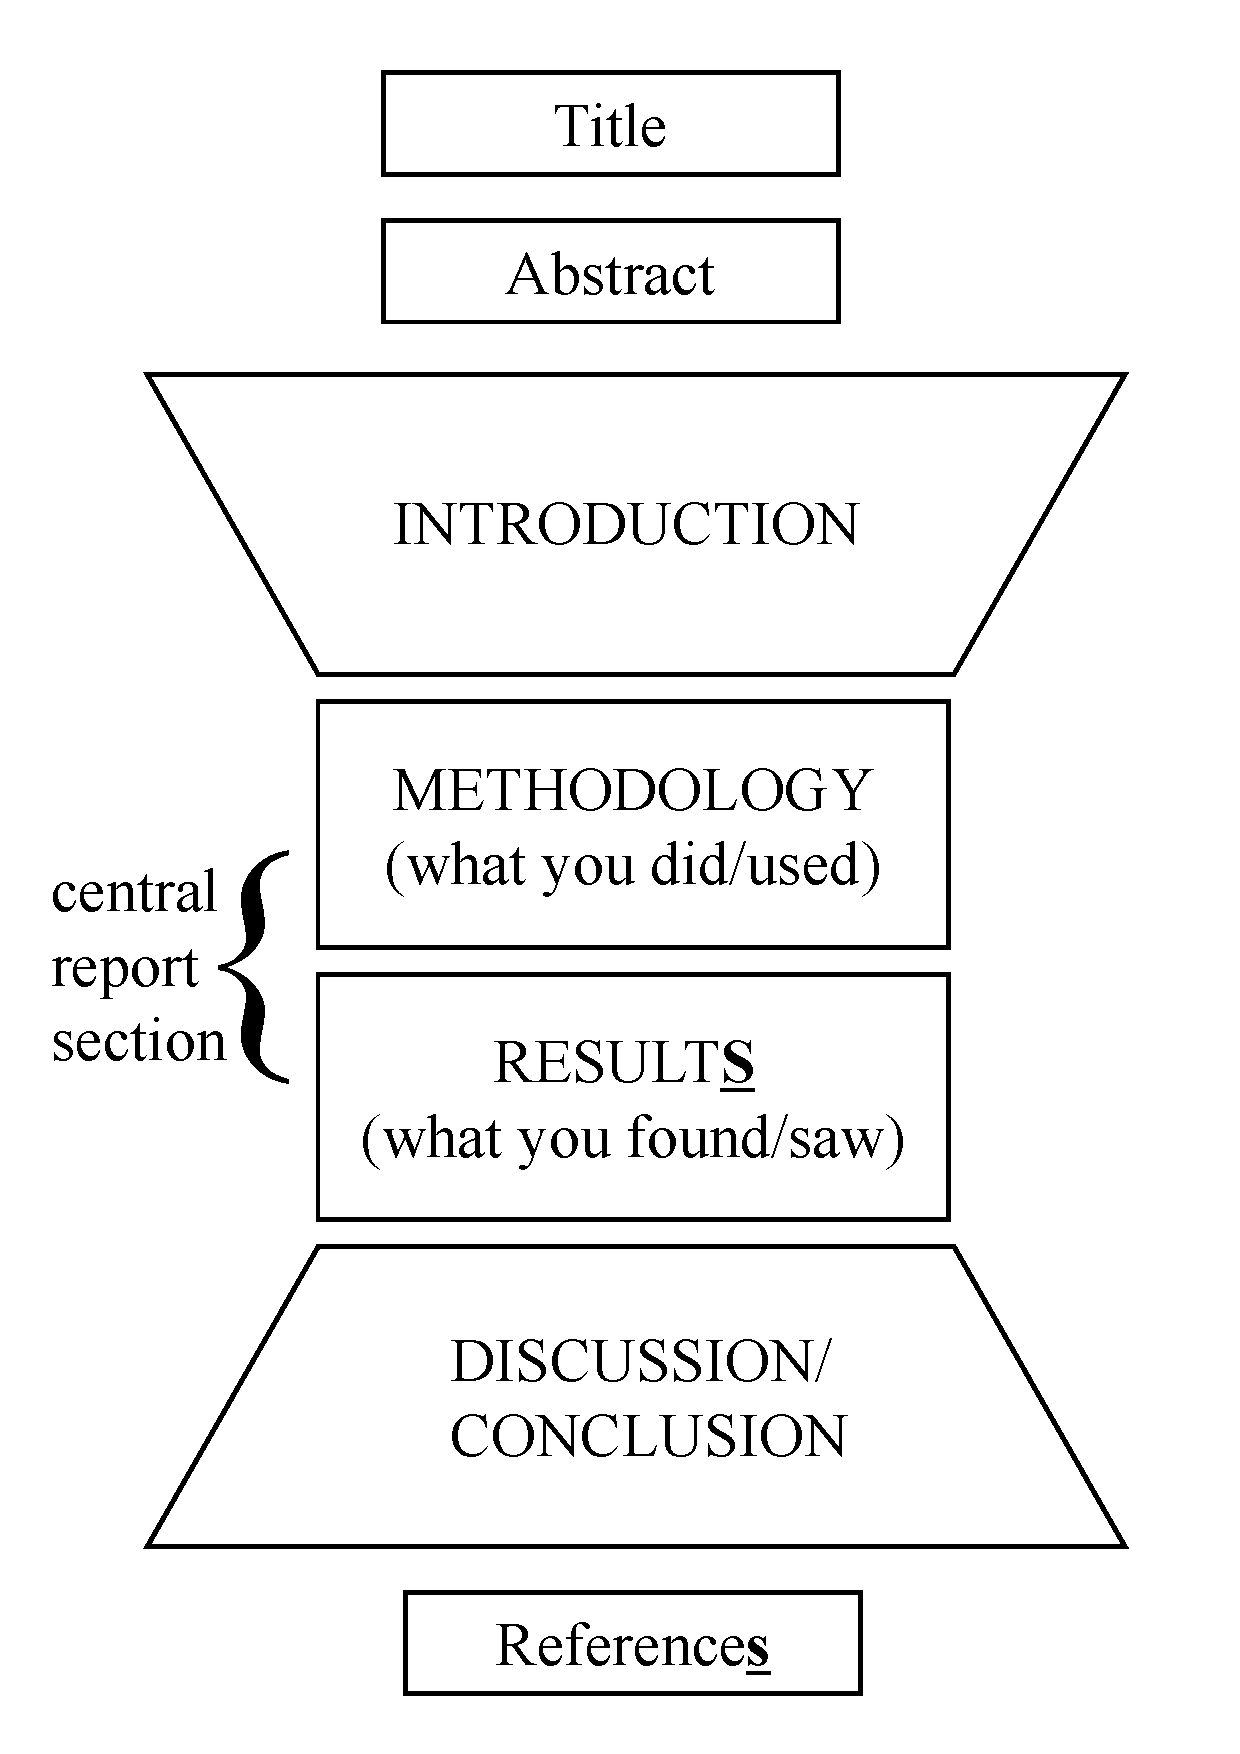
\includegraphics[width=0.65\textwidth]{structure_v3.pdf}
	\end{figure}
	이 정리노트는 2015학년도 2학기에 진행된 경기과학고등학교 류지석 선생님의 `영어논문작성법' 수업, `Science Research Writing for Non-Native Speakers of English(Hilary Glasman-Deal, Imperial College Press)' 책을 기반으로 제작되었습니다.
	%% 크리에이티브 커먼즈 표시를 하기에는 문서 내용이 책에서 가져온 것이 많아 조금 문제가 있다고 판단하였습니다. 저작권 관련해서 잘 아는 사람이 확인한 다음 다시 달아주시기 바랍니다.
	%% 아니 이걸 당연히 달면 안 되죠. 원저작자가 아닌데 ㅁㄴㅇㄹ
	%% ㅠㅠ
	
	
	%% for reducing space above title of chapter
	\titleformat{\chapter}[display]
	{\normalfont\huge\bfseries}{\chaptertitlename\ \thechapter}{20pt}{\Huge}
	\titlespacing*{\chapter}
	{0pt}{-20pt}{40pt}
	%%
	
	
	\tableofcontents
	\addcontentsline{toc}{chapter}{Table of Contents}
	%% \listoftables %% 굳이 필요 없는 것 같아서 일단 제거.
	%% \addcontentsline{toc}{chapter}{List of Tables}
	
	\chapter{Introduction}
	
	\section{Grammar}
	
	\subsection{Active vs Passive} \label{intro_grammar_active_passive}
	보통 문장을 능동태로 쓰면 독자는 행위의 대상(논문의 내용)이 아닌 행위의 주체(논문의 저자 - I, we)에 초점을 두고 읽게 된다. 반면 수동태를 쓸 경우 행위의 주체를 생략할 수 있으므로(이를 agentless passive라 한다.) 독자가 논문의 내용에 집중할 수 있게 된다. 때문에, 과학 논문에서는 능동태보다는 수동태를 쓰는 것이 권장된다. 이 내용은 \ref{method_grammar_active_passive}절에서 이어진다.
	
	\begin{comment}
	
	\section{Writer's intention}
	(이미 시험을 봤기 때문에 출제되지 않음)
	\begin{enumerate} % p24에 열거되어 있지만 요약된 버전이라서 요약 없이 여기에 열거함
	\item The writer establishes the importance of this research topic.
	\item ... provides general background information for the reader.
	\item ... does the same as in 1 and 2, but in a more specific/detailed way, using research references to support both the background facts and the claim for significance.
	\item ... describes the {\it general problem} area or the current research focus of the field. (\bf `However')
	\item ... provides a transition between the general problem area and the {\it literature review}.
	\item ... provides a brief overview of key research projects in this area.
	\item ... describes a gap in the research. ({\it specific problems})
	\item ... describes the paper itself.
	\item ... gives details about the methodology reported in the paper.
	\item ... announces the findings.
	\end{enumerate}
	\end{comment}
	
	\section{Sentences / Vocabulary}
	\begin{itemize}
		\item (pp.35) Nanocrystalline oxide films {\bf are attracting widespread interest} in fields such as nanoelectronics.\\
		해석 : 나노결정 산화 필름은 나노전자공학과 같은 분야에서 넓은 관심을 끌고 있다.
		\item (pp.35) {\bf The importance of} strength anisotropy has been demonstrated by the institute.\\
		해석 : 강도 이방성의 중요함은 그 연구소에 의해 입증되어 왔다.
		\item (pp.37) In their study, expanded T-cells {\bf were found} in two cases, respectively.\\
		해석 : 그들의 연구에서는, 팽창된 T 세포들이 두 경우에서 각각 발견되었다.
		\item (pp.37) Initial attempts {\bf focused on identifying} the cause of the problems.\\
		해석 : 초기의 연구들은 그 문제들의 원인을 확인하는 것에 초점을 맞추었다. \\
		유의 : attempt를 시도보다는 연구로 해석하는 것이 더 어울립니다.
		\item (pp.39) However, light scattering techniques have been {\bf largely unsuccessful} to date.\\
		해석 : 그러나, 빛 산란 기술은 오늘에 이르기까지 주로 성공적이지 못했다. \\
		유의 : largely를 `주로'라고 해석하였습니다.
		\item (pp.39) {\bf Although} this approach improves performance, it results in an unacceptable number of machine failures.\\
		해석 : 이 접근법이 성능을 향상시킴에도 불구하고, 그것은 용납할 수 없을 만큼 많은 기계 오작동을 낳는다.\\
		유의 : a(an) number of : 많은, the number of : -의 수
		\item (pp.40) {\bf This paper focuses on} reducing the power consumption of wireless microsensor networks. \\
		해석 : 본 논문은 무선 마이크로 네트워크의 전력 소비 감소에 집중한다.
	\end{itemize}
	\chapter{Methodology}
	
	\section{Grammar}
	
	\subsection{Active vs Passive} \label{method_grammar_active_passive}            
	(\ref{intro_grammar_active_passive}절에서 이어짐)
	우리가 과학 논문을 작성할 때, 연구 팀에 속한 채로 논문을 작성할 때는 논문을 작성하는 주체가 `we' 이다. 이 경우 상황에 따라 논문의 문장을 능동태로 작성해도 될 때가 있다. 하지만 박사학위 논문과 같이 혼자 쓰는 논문의 경우, 논문을 작성하는 주체가 `I'와 같이 1인칭 단수이므로 쓰지 않는 것이 좋다(고 책 pp.47에 나와있다.)
	%% 말줄임표가 들어가야 할 부분이 아닌 것 같아 괄호 처리하였습니다.
	
	\subsection{Present vs Past}
	\begin{itemize}
		\item {\it A flexible section is inserted in the pipe.} : Present Simple passive \\
		보편적으로 널리 알려진 방법/절차 : present 사용
		\item {\it A flexible section was inserted in the pipe.} : Past Simple passive \\
		우리가 진행한 연구만의 독특한 방법/절차 : past 사용
	\end{itemize}
	남들이 이미 연구한 내용과, 우리가 연구하거나 독창적으로 수행한 것이 이와 같이 present / past 를 통해 제대로 구분되지 않는다면 그것은 \textbf{disaster}이다!
	
	\subsection{The}
	The를 쓰는 경우는, phrase 같은 것들이 아니라면 다음과 같이 2가지가 있다.
	\begin{enumerate}
		\item When you and your reader both know which thing/person you mean.\\
		{\it e.g.} I had a cheese sandwich and an apple for lunch. {\bf The} sandwich was fine but {\bf the} apple had a worm in it.
		\item When there is only one possible referent.
		{\it e.g.} {\bf The} sun rises in {\bf the} east.
	\end{enumerate}
	
	\subsection{The vs A}
	선생님께서 여기에서는 출제하지 않았다고 하셨다.
	
	\section{Writer's intention}
	(이미 시험을 봤기 때문에 출제되지 않음)
	
	\section{Sentences / Vocabulary}
	\begin{itemize}
		\item (pp.78) {\bf The impact tests used in this work} were a modified version of the previous one. \\
		해석 : 이번 연구에서 사용된 충격 시험은 이전 \textit{방법}의 변형판이었다. \\
		유의 : `previous one'의 one 은 version 과 같은 뜻.
		\item (pp.79) Porosity was measured {\bf at the near end and at the far end} of the polished surface. \\
		%polish는 윤내다, 광택을 내다라는 뜻입니다.
		해석 : 광택면의 가까운 쪽의 끝과 먼 쪽의 끝에서 다공성이 측정되었다.
		\item (pp.80) Similar loads were applied to {\bf the front and side} of the box. \\
		%해석 : 비슷한 하중이 상자의 앞과 옆에 가해졌다.
		해석 : 상자의 앞과 옆에 비슷한 하중이 가해졌다. \\
		유의 : loads가 하중이라는 뜻을 가집니다.
		\item (pp.83) (어려움) Zinc oxide was drawn into the laminate {\bf with the intention of} enhancing delaminations and cracks. \\
		%해석1 : 산화 아연 박편은 얇은막갈라짐(delamination)과 균열(crack)을 늘리기 위해 laminate로 draw 되었다?\\
		%해석2 : 산화 아연이 균열을 늘리기 위한 목적으로 합판 안에 추가되었다.\\
		해석 : 산화 아연이 엽열과 균열을 늘리기 위한 목적으로 박편으로 만들어졌다.
		\item (pp.83) {\bf The advantage of} using three-dimensional analysis was that the out-of-plane stress field could be obtained. \\
		해석 : 3차원 분석을 사용하는 것의 장점은 면 바깥의 압력장을 구할 수 있다는 것이었다.
		\item (pp.84) After being removed, the mouse lungs were frozen and thawed {\bf at least} three times. \\
		해석 : 쥐의 폐는 적출된 이후에 적어도 세 번은 냉동되고 해동되었다.
		\item (pp.86) In our implementation {\bf we followed} Sato {\it et al.} (1998) by using a discrete kernel size. \\
		해석 : 우리의 실행에서는 개별적인 핵의 크기를 이용함으로써 Sato 등을 따라하였다. \\
		유의 : implementation을 `실행'이라고 해석하였습니다. 출처는 작년 시험지.
		\item (pp.87) Only a brief observation was feasible, {\bf however,} given the number in the sample. \\
		해석 : 그러나, 표본의 개수를 감안하면, 간단한 관측만이 가능했다. \\
		유의 : given이 considering의 뜻으로 사용되었습니다.
		\item (pp.87) {\bf Although} centrifugation could not remove all the excess solid drug, the amount remaining was negligible. \\
		해석 : 비록 원심 분리가 모든 초과한 고체 약품을 제거할 수는 없었지만, 남아있는 양은 무시 가능한 수준이었다.
	\end{itemize}
	
	\chapter{Results}
	
	\section{Grammar}
	
	\subsection{Communicate sequence}
	뭔가 해석하기 애매모호한데, 간단히 접속사라고 생각하자. 관련 예문은 \ref{practice_phrases} 장에 있다.
	\begin{itemize}
		\item afterwards : 나중에
		\item in advance : 사전에, 미리
		\item in the meantime : 한편, 그 동안
		\item simultaneously : 동시에, 일제히
		\item subsequently : 뒤이어
		% 전 이거랑 consequently랑 헷갈리더군요. 이건 '결과적으로'라는 뜻입니다.
	\end{itemize}
	
	\subsection{Adverbs of frequency}
	흔히 `빈도부사'라고 불리는 것들이다. WGRFMAOORSO
	\begin{table}[ht!]
		\centering
		\begin{tabular}{|l|l|}
			\hline
			Frequency & Phrase \\ \hline
			100~\%         &   without exception     \\ \hline
			&   generally     \\ \hline
			&   regularly    \\ \hline
			&   frequently     \\ \hline
			&   more often than not     \\ \hline
			50~\%      &   as often as not ({\bf neutral frequency})\\ \hline
			&   on some occasions     \\ \hline
			&   occasionally     \\ \hline
			&   rarely    \\ \hline
			&   scarcely ever     \\ \hline
			0~\%       &   on no occasion     \\ \hline
		\end{tabular}
		\caption{Adverbs of Frequency}
		\label{adverbs_of_frequency}
	\end{table}
	\clearpage
	\subsection{Phrases of quantity}
	양에 관한 몇 개의 어구들이다. 관련 예문은 \ref{practice_phrases} 장에 있다.
	\begin{table}[ht!]
		\centering
		\begin{tabular}{|l|l|l|}
			\hline
			Category                  & Phrase          &  Definition   \\ \hline
			\multirow{2}{*}{Increase} & a great deal (of) & 많은 \\ \cline{2-3} 
			& considerable & 많은      \\ \hline
			\multirow{2}{*}{Reduce}   & infinitesimal & 극미량의   \\ \cline{2-3} 
			& marginal   & 불충분한      \\ \hline
			Emphasize                 & exceptionally & 예외적으로     \\ \hline
		\end{tabular}
		\caption{Phrases of Quantity}
		\label{phrases_of_quantity}
	\end{table}
	
	\section{Writer's intention}
	(출제되지 않음)
	
	\section{Sentences / Vocabulary}
	\begin{itemize}
		\item (pp.137) {\bf Since} the angular alignment is critical, the effect of an error in orientation was {\bf investigated experimentally.} \\
		해석 : 각 정렬이 중요하기 때문에, 위치에 있어서의 오차의 효과는 실험적으로 조사되었다.
		\item (pp.137) {\bf It was suggested in the Introduction } that the effective stress paths may be used to define local bounding surfaces. \\
		해석 : 효과적인 응력 경로들이 국부적인 결합 표면을 정의하는데 쓰일 수도 있다는 것이 서론에서 제안되었다.
		\item (pp.138) {\bf It is evident} that these results are in good agreement with their FE counterparts. \\
		해석 : 이러한 결과들은 그들의 FE 대응물과 잘 일치한다는 것이 명백하다.
		\item (pp.139) The stress data in Fig. 18 {\bf indicate} a more reasonable relationship. \\
		해석 : 그림 18의 응력 자료는 더 타당한 관련성을 보여 준다.
		\item (pp.139) {\bf Comparing Figs. 1 and 4} shows that volumetric strains developed after pore pressure had dissipated. \\
		해석 : 그림 1과 4의 비교는 기공 압력이 사라진 이후에 부피 응력이 발달되었다는 것을 보여 준다.
		\item (pp.141) There was a {\bf lower} proportion of large particles present at lower pH. \\
		해석 : 낮은 pH에 존재하던 큰 입자의 비율이 낮았다.
		\item (pp.142) Comparing Figs. 4 and 5, it is obvious that a {\bf significant} improvement was obtained in {\bf the majority of} cases. \\
		해석 : 그림 4와 5를 비교하면, 대부분의 경우에서 상당한 진전이 얻어졌다는 것은 명백하다.
		\item (pp.144) These trends are {\bf in line with} the previously discussed structure of the ferrihydrite aggregates. \footnote{책의 of the 2번은 오타} \\
		해석 : 이 경향들은 이전에 논의된 ferrihydrite 골재의 구조와 일치한다.
		\item (pp.145) {\bf Although} this was {\bf not} obtained experimentally, it can be assumed to exist. \\
		해석 : 비록 이것이 실험적으로 얻어지지는 않았지만, 그것은 존재한다고 가정될 수 있다.
		\item (pp.149) {\bf It could be inferred} therefore that these {\bf may have} reacted with ozone to form organic acids, such as formic acid. \\
		%해석 : 우리는 이로부터 이것들이 오존과 반응하여 폼산과 같은 유기산을 형성할 수 있었다는 것을 추론할 수 있다. \\
		해석 : 그러므로 이것들이 오존과 반응하여 폼산과 같은 유기산들을 형성했는지도 모른다는 것이 추론될 수 있다. \textbackslash\textbackslash 위 해석에 therefore가 없어서. 수동태는 의역하지 않고 수동태로 해석. \\
		유의 : can have P.P 를 may have P.P 와 구별할 것.
	\end{itemize}
	
	\chapter{Discussion / Conclusion}
	
	\section{Modal Verbs}%조동사라는 뜻입니다. model이 아니라고!
	수업시간에 modal sentence들에 관해 배우고, 표 \ref{modal_table}과 같은 예시 6가지와 그 한국어 의미를 배웠습니다. (교재 pp.166)
	\begin{table}[ht]
		\centering
		\begin{tabular}{c||c|c|c}
			\hline
			may have P.P & -했을지도 모른다 & 과거의 약한 추측 & $\fallingdotseq$ might have P.P\\
			\hline
			can have P.P & -할 수 있었을 것이다 & 과거의 가능성 & \\
			\hline
			would have P.P & -했을 것이다 & 과거의 의지 & \\
			\hline
			must have P.P & -했음에 틀림없다 & 과거의 강한 추측 & \\
			\hline
			should have P.P & -했어야 한다 & 과거의 유감 & $\longleftrightarrow$ should not have P.P \\
			\hline
			cannot have P.P & -했을리가 없다 & 과거의 강한 부정추측 & \\
			\hline
		\end{tabular}
		\caption{Modal Sentences}
		\label{modal_table}
	\end{table}
	P.P 자리에 be 동사가 오는 경우에는 당연하지만  `했음' 이 `이었음' 처럼 바뀐다.
	\begin{figure}[ht]
		\centering
		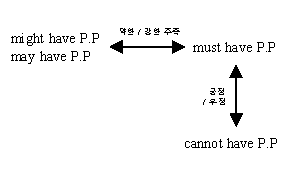
\includegraphics[width=0.7\textwidth]{modal.pdf}
		\caption{여러 modal sentences 간의 관계}
		\label{modal_relation}
	\end{figure}
	
	\section{Writer's intention}
	\textbf{반드시 외워야 함.}
	\begin{enumerate}
		\item The writer revisits previous research.
		\item ... revisits the Introduction to recall specific weakness in the methodology used in previous studies.
		\item ... revisits the methodology used in this study.
		\item ... revisits and summarises the results.
		\item ... shows where and how the present work fits into the research `map' in this field.
		\item ... recalls an aspect of the results that represents a positive achievement or contribution of this work.
		\item ... focuses on the meaning and implications of the achievements in this work.
		\item ... notes that one of the achievements or contributions of this work is its novelty.
		\item ... refines the implications of the results, including possible applications.
		\item ... describes the limitations which should direct future research.
		\item ... suggests a specific area to be addressed in future work.
	\end{enumerate}
	
	\section{Sentences / Vocabulary}
	\begin{itemize}
		\item (pp.189) {\bf To the knowledge of authors,} the data in Figs. 4-6 is the {\bf first of its kind in the treatment of appendicitis}. \\
		해석 : 저자들의 지식에 의하면, 그림 4-6의 자료는 맹장염의 치료에 있어서는 그 분야의 처음의 것이다. 
		\item (pp.189) Our results are {\bf in general agreement with} previous morphometric and DNA incorporation studies in the rat [2.6]. \\
		해석 : 우리의 결과들은 쥐에 관련된 이전의 형태적이고 DNA 합성에 관한 연구와 대체로 일치한다. \\
		유의 : morphometric : 형태적(morpho-) 측정(metric) \\
		의문 : DNA incorporation : 생올러 아무나 해석 좀......
		\item (pp.192) An important question for {\bf future studies} is to determine the antidepressant effects of such drugs. \\
		해석 : 후속 연구를 위한 중요한 과제는 이러한 약물들의 항우울 효과를 측정하는 것이다. \\
		유의 : determine - 결정/측정, 측정 - measure/determine
		\item (pp.193) Our technique {\bf can be applied to} a wide range of simulation applications. \\
		해석 : 우리의 기술은 광범위한 모의 실험 응용들에 적용될 수 있다.
		\item (pp.193) The PARSEX reactor therefore could be {\bf used} for the realistic testing of a wide range of control algorithms. \\
		해석 : 따라서 PARSEX 리액터는 넓은 범위의 제어 알고리즘의 현실적인 시험에 사용될 수 있을 것이다. \\
		유의 : 리액터가 여러 의미가 있으나 전기·전자 분야에서는 번역어가 딱히 없음
	\end{itemize}
	\chapter{Abstract}
	
	\section{Definition}
	\Large Abstract is a \underline{\textbf{summary}} of a paper in a concrete, concise, and specific manners using 150-250 words.
	\normalsize
	
	\section{Writer's intention(MODEL 1)}
	\textbf{이것도 반드시 외워야 함.}
	\begin{enumerate}
		\item The writer provides background factual information.
		\item ... combines the method, the general aim and the specific aim of the study in one sentence.
		\item ... summarises the methodology and provides details.
		\item ... indicates the achievement of the study.
		\item ... presents the implications of the study.
	\end{enumerate}
	
	\section{Sentences / Vocabulary}
	우리가 불쌍해서 안 넣으셨다고 한다.
	
	\appendix
	\chapter{Abbreviations Used in Science Writing}
	\begin{table}[ht!]
		\centering
		\def\arraystretch{1.3} %vertical padding
		\begin{tabular}{|l|l|l|}
			\hline
			Abbreviation & Full word/phrase & Meaning \\ \hline
			\textit{c.} (or \textit{ca.})  &    \textit{circa}    &    \begin{tabular}[c]{@{}l@{}}about\\ approximately \\around \end{tabular}\\  \hline
			\textit{cf.}&       \textit{confer}  &  compare   \\ \hline
			\textit{et al.}&    \textit{et alii} &    and others  \\ \hline
			\textit{vs.}&  \textit{versus} &  \begin{tabular}[c]{@{}l@{}}as opposed to\\ against \\in contrast to \end{tabular}  \\ \hline
			\textit{i.e.}&   \textit{id est}  &  \begin{tabular}[c]{@{}l@{}}that is\\ in other words \end{tabular}   \\ \hline
			\textit{e.g.}&    \textit{exempli gratia}  & for example \\ \hline
			\textit{N.B.}&  \textit{nota bene}  & \begin{tabular}[c]{@{}l@{}} please note\\ note well \end{tabular}  \\ \hline
			\textit{p.a.}& \textit{per annum} & \begin{tabular}[c]{@{}l@{}} per year\\ yearly \end{tabular}  \\ \hline
		\end{tabular}
		\caption{Abbreviations Used in Science Writing}
		\label{appendix_1}
	\end{table}
	\vskip 0.5cm
	Test format : 가운데 로마어 어구만 주고, 이를 어떻게 줄여쓰며 의미는 무엇인지를 써야 합니다.\\
	Some facts : 마침표(.)는 이 단어가 축약되었다는 것을 의미합니다.
	\stepcounter{chapter}
	\chapter{Some Singular and Plural Forms}
	\begin{table}[ht!]
		\centering
		\def\arraystretch{1.0} %vertical padding
		\begin{tabular}{|l||l|l|l|}
			\hline
			\textbf{Type} & Singular & Plural & Definition \\
			\hline
			\hline
			\begin{tabular}[c]{@{}l@{}} \textbf{A} \\ -a $\rightarrow$ -ae \end{tabular} & 
			\begin{tabular}[c]{@{}l@{}} alga \\ antenna \\ formula \\ vertebra \end{tabular} &   
			\begin{tabular}[c]{@{}l@{}} algae \\ antennae \\ formulae \\ vertebrae \end{tabular} &
			\begin{tabular}[c]{@{}l@{}} 조류 \\ 더듬이 \\ 공식 \\ 척추골 \end{tabular}
			\\  \hline
			\begin{tabular}[c]{@{}l@{}} \textbf{B} \\ -is $\rightarrow$ -es \end{tabular} & 
			\begin{tabular}[c]{@{}l@{}} analysis \\ axis \\ basis \\ crisis \\ diagnosis \\ hypothesis \\ psychosis \\ thesis \end{tabular} &   
			\begin{tabular}[c]{@{}l@{}} analyses \\ axes \\ bases \\ crises  \\ diagnoses \\ hypotheses \\ psychoses \\ theses \end{tabular} &
			\begin{tabular}[c]{@{}l@{}} 분석 \\ 축 \\ 기본 \\ 위기 \\ 진단 \\ 가설 \\ 정신병 \\ 논문 \end{tabular}
			\\  \hline
			\begin{tabular}[c]{@{}l@{}} \textbf{C} \\ -um/-on $\rightarrow$ -a \end{tabular} & 
			\begin{tabular}[c]{@{}l@{}} bacterium \\ criterion \\ curriculum \\ datum \\ medium \\ ovum \\ phenomenon \\ serum \\ spectrum \end{tabular} &   
			\begin{tabular}[c]{@{}l@{}} bacteria \\ criteria \\ curricula \\ data \\ media \\ ova \\ phenomena \\ sera \\ spectra \end{tabular} &
			\begin{tabular}[c]{@{}l@{}} 병원균 \\ 기준 \\ 교육과정 \\ 자료 \\ 매체 \\ 난자 \\ 현상 \\ 혈청 \\ 스펙트럼 \end{tabular}
			\\  \hline
			\begin{tabular}[c]{@{}l@{}} \textbf{D} \\ -ex/-ix $\rightarrow$ -ices \end{tabular} & 
			\begin{tabular}[c]{@{}l@{}} appendix \\ index \\ matrix \\ vortex \end{tabular} &   
			\begin{tabular}[c]{@{}l@{}} appendices \\ indices \\ matrices \\ vortices \end{tabular}&
			\begin{tabular}[c]{@{}l@{}} 막창자꼬리 \\ 지표 \\ 자궁, 행렬 \\ 회오리 \end{tabular} 
			\\ \hline
			\begin{tabular}[c]{@{}l@{}} \textbf{E} \\ -us $\rightarrow$ -i \end{tabular} & 
			\begin{tabular}[c]{@{}l@{}} locus \\ nucleus \\ radius \\ stimulus \end{tabular} &   
			\begin{tabular}[c]{@{}l@{}} loci \\ nuclei \\ radii \\ stimuli \end{tabular}&
			\begin{tabular}[c]{@{}l@{}} 자취 \\ 핵 \\ 반지름 \\ 자극 \end{tabular} 
			\\ \hline
			\textbf{Exc)} & genus & genera & 종
			\\ \hline
		\end{tabular}
		\caption{Latin and Greek Singular and Plural Forms}
		\label{appendix_3}
	\end{table}
	
	\chapter{Practice : Sentences}
	안타깝게도 시험 양식이 \sout{의미 없는 몇 개의 영어 어휘들을 보고} 주어진 한글 문장에 맞게 책에 있는 영어 문장을 기입하는 것이므로, 이렇게 번역된 문장만 있는 chapter를 부득이하게 만듭니다. 그나마 희망스러운 건 작년 시험의 경우 거의 순서대로 나왔다는 것.
	\begin{itemize}
		\item 나노결정 산화 필름은 나노전자공학과 같은 분야에서 넓은 관심을 끌고 있다.
		\item 강도 이방성의 중요함은 그 연구소에 의해 입증되었다.
		\item 그들의 연구에서는, 팽창된 T 세포들이 두 경우에서 각각 발견되었다.
		\item 초기의 연구들은 그 문제들의 원인을 확인하는 것에 초점을 맞추었다.
		\item 그러나, 빛 산란 기술은 오늘에 이르기까지 주로 성공적이지 못했다.
		\item 이 방법이 성능을 향상시킴에도 불구하고, 그것은 용납할 수 없을 만큼의 기계 오작동을 낳았다.
		\item 본 논문은 무선 마이크로 네트워크의 전력 소비 감소에 집중한다.
		\item 이번 연구에서 사용된 충격 시험은 이전 방법의 변형판이었다.
		\item 광택면의 가까운 쪽의 끝과 먼 쪽의 끝에서 다공성이 측정되었다.
		\item 상자의 앞과 옆에 비슷한 하중이 가해졌다.
		\item 산화 아연이 엽열과 균열을 늘리기 위한 목적으로 박편으로 만들어졌다.
		\item 3차원 분석을 사용하는 것의 장점은 면 바깥의 압력장을 구할 수 있다는 것이었다.
		\item 쥐의 폐는 적출된 이후에 적어도 세 번은 냉동되고 해동되었다.
		\item 우리의 실행에서는 개별적인 핵의 크기를 이용함으로써 Sato 등을 따라하였다.
		\item 그러나, 표본의 개수를 감안하면, 간단한 관측만이 가능했다.
		\item 비록 원심 분리가 모든 초과한 고체 약품을 제거할 수는 없었지만, 남아있는 양은 무시 가능한 수준이었다.
		\item 각 정렬이 중요하기 때문에, 위치에 있어서의 오차의 효과는 실험적으로 조사되었다.
		\item 효과적인 응력 경로들이 국부적인 결합 표면을 정의하는데 쓰일 수도 있다는 것이 서론에서 제안되었다.
		\item 이러한 결과들은 그들의 FE 대응물과 잘 일치한다는 것이 명백하다.
		\item 그림 18의 응력 자료는 더 타당한 관련성을 보여 준다.
		\item 그림 1과 4의 비교는 기공 압력이 사라진 이후에 부피 응력이 발달되었다는 것을 보여 준다. % 공극내 압력 아닌가가요?? 
		\item 낮은 pH에서 존재하는 큰 입자의 비율이 낮았다.
		\item 그림 4와 5를 비교하면, 대부분의 경우에서 상당한 진전이 얻어졌다는 것은 명백하다.
		\item 이 경향들은 이전에 논의된 ferrihydrite 골재의 구조와 일치한다.
		\item 비록 이것이 실험적으로 얻어지지는 않았지만, 그것은 존재한다고 가정될 수 있다.
		\item 그러므로 이것들이 오존과 반응하여 폼산과 같은 유기산들을 형성했는지도 모른다는 것이 추론될 수 있다.
		\item 저자들의 지식에 의하면, 그림 4-6의 자료는 맹장염의 치료에 있어서는 그 분야의 처음의 것이다. 
		\item 우리의 결과들은 이전에 이루어진 쥐의 형태적 측정 및 DNA incorporation 연구와 대체로 일치한다.
		\item 후속 연구를 위한 중요한 과제는 이러한 약물들의 항우울 효과를 측정하는 것이다.
		\item 우리의 기술은 광범위한 모의 실험 응용들에 적용될 수 있다.
		\item 따라서 PARSEX 리액터는 넓은 범위의 제어 알고리즘의 현실적인 시험에 사용될 수 있을 것이다.
	\end{itemize}
	
	\chapter{Practice : Phrases}\label{practice_phrases}
	교과서에 마땅한 예문도 없는데 작년 시험에는 영작하라고 나왔으니 뭐 할 말이 없네요. 그래도 ``영작해보세요!''라고 예문을 몇 개 드리겠습니다. \\
	주의사항 : 작년의 경우, 8단어 이상으로 문법적 오류가 없으면서 어색하지 않게 영작을 해야 했습니다.
	\begin{itemize}
		%\itemsep 0em
		\item afterwards, velocity, increased
		%The target's average velocity has increased afterwards.
		\item in advance, complexity, calculated
		%The complexity of the algorithm was calculated in advance.
		\item in the meantime, solution, cooled down
		%In the meantime, the solution was cooled down for further experiments.
		\item simultaneously, objects, hit, ground
		%Surprisingly, the objects simultaneously hit the ground.
		\item subsequently, bacteria, cloned
		%Subsequently, the bacteria did not cloned themselves.
		\item a great deal of, damage, failure
		%A great deal of damage eventually resulted the machine's failure.
		\item considerable, cost, experiment
		%Considerable amount of cost is required to perform this experiment.
		\item infinitesimal, cells, body
		%There are trillions of infinitesimal cells in our body.
		\item marginal, error, estimation
		%The is an error in our estimation, but its scale is marginal.
		\item exceptionally, angle, collision
		%There were some exceptionally high angles during the collision test.
	\end{itemize}
	예시는 다음 장에 나와 있습니다.
	\newpage
	\begin{itemize}
		%\itemsep 0em
		\item The target's average velocity has increased afterwards.
		\item The complexity of the algorithm was calculated in advance.
		\item In the meantime, the solution was cooled down for further experiments.
		\item Surprisingly, the objects simultaneously hit the ground.
		\item Subsequently, the bacteria did not cloned themselves.
		\item A great deal of damage eventually resulted the machine's failure.
		\item Considerable amount of cost is required to perform this experiment.
		\item There are trillions of infinitesimal cells in our body.
		\item There is an error in our estimation, but its scale is marginal.
		\item There were some exceptionally high angles during the collision test.
	\end{itemize}
	
	\chapter{Practice : Writer's Intention}
	%책을 펼칠 필요도 없게 만드는 대단한 학습지 %% ㅁㄴㅇㄹ
	Model Discussion \& Conclusion입니다. 참고로 10번 문장과 11번 문장의 의도는 같습니다.
	\begin{quote}
		{\bf 1} Prior work has documented the effectiveness of psychosocial intervention in improving quality of life (QoL) and reducing stress in patients suffering from various disorders; Epstein,$^{18}$ for example, reports that orthopedic patients participating in a two-week multimedia intervention programme improved across several QoL indices, including interpersonal conflict and mental health. {\bf 2} However, these studies have either been short-term studies or have not focused on patients whose disorder was stress-related. {\bf 3} In this study we tested the extent to which an extended three-month stress management programme improved QoL among a group of patients being treated for stress-related skin disorders such as eczema. {\bf 4} We found that in virtually all cases, participation in our three-month stress management programme was associated with substantial increases in the skills needed to improve QoL. {\bf 5} These findings extend those of Kaliom, confirming that a longer, more intensive period of stress-management training tends to produce more effective skills than when those skills are input over a shorter period via information transfer media such as leaflets and presentations (Kaliom {\it et al.}, 2003). {\bf 6} In addition, the improvements noted in our study were unrelated to age, gender or ethnic background. {\bf 7} This study therefore indicates that the benefits gained from stress-management intervention may address QoL needs across a wide range of patients. {\bf 8} Most notably, this is the first study to our knowledge to investigate the effectiveness of extended psychosocial intervention in patients whose disorder is itself thought to be stress-related. {\bf 9} Our results provide compelling evidence for long-term involvement with such patients and suggest that this approach appears to be effective in counteracting stress that may exacerbate the disorder. {\bf 10} However, some limitations are worth noting. {\bf 11} Although our hypotheses were supported statistically, the sample was not reassessed once the programme was over. {\bf 12} Future work should therefore include follow-up work designed to evaluate whether the skills are retained in the long term and also whether they continue to be used to improve QoL.
	\end{quote}
	\newpage
	이쪽은 Model Abstract (1)입니다. 참고로 3번 문장과 4번 문장의 의도는 같습니다.
	\begin{quote}
		{\bf 1} The speed of sound in a fluid is determined by, and therefore an indicator of, the thermodynamic properties of that fluid. {\bf 2} The aim of this study was to investigate the use of an ultrasonic cell to determine crude oil properties, in particular oil density. {\bf 3} An ultrasonic cell was constructed to measure the speed of sound and tested in a crude oil sample. {\bf 4} The speed of sound was measured at temperatures between 260 and 411 K at pressures up to 75 MPs. {\bf 5} The measurements were shown to lead to an accurate determination of the bubble point of the oil. {\bf 6} This indicates that there is a possibility of obtaining fluid density from sound speed measurements and suggests that it is possible to measure sound absorption with an ultrasonic cell to determine oil viscosity.
	\end{quote}
\end{document}